\section{随机变量及其分布}

\begin{question}{补充习题}
    设某便利店一天中的顾客人数服从参数为 10 的泊松分布,并且这些到店顾客的购物行为彼此独立,其购物概率为 0.6,求每天到便利店且购物的顾客人数的分布.
\end{question}
\begin{solution}
    我们约定用随机变量 $X$ 表示到店的人数,$Y$ 表示到店且购物的人数. 设当天有 $r (r=0, 1, 2, \cdots)$位顾客到店,其中 $k (k \leqslant r)$ 位顾客在到店后选择购物,那么
    $$
        P\{Y=k|X=r\} = C_r^k(0.6)^k(1-0.6)^{r-k}.
    $$
    再根据全概率公式
    $$
        \begin{aligned}
            P\{Y=k\}
             & = \sum_{r=k}^{\infty} P\{Y=k|X=r\} P\{X=r\}                                                 \\
             & = \sum_{r=k}^{\infty} C_r^k(0.6)^k(1-0.6)^{r-k} \frac{10^r\mathrm{e}^{-10}}{r!}             \\
             & = \sum_{r=k}^{\infty} \frac{r!}{k!(r-k)!}(0.6)^k(0.4)^{r-k}\frac{10^r\mathrm{e}^{-10}}{r!}. \\
        \end{aligned}
    $$
    约去 $r!$ 后,进一步令 $r-k=i$
    $$
        \begin{aligned}
            P\{Y=k\}
             & = \sum_{i=0}^{\infty} \frac{1}{k!i!}(0.6)^k(0.4)^{i}10^{i+k}\mathrm{e}^{-10}  \\
             & = \frac{0.6^k10^k\mathrm{e}^{-10}}{k!}\sum_{i=0}^{\infty}\frac{0.4^i10^i}{i!} \\
             & = \frac{6^k\mathrm{e}^{-10}}{k!} \sum_{i=0}^{\infty}\frac{4^i}{i!}            \\
             & = \frac{6^k\mathrm{e}^{-6}}{k!}.
        \end{aligned}
    $$
\end{solution}

\begin{question}{题目2}
    \begin{itemize}
        \item [(1)] 一袋中装有 5 只球,编号为 1,2,3,4,5. 在袋中同时取 3 只,以 $X$ 表示取出的 3 只球中的最大号码,写出随机变量 $X$ 的分布律.
        \item [(2)] 将一颗骰子抛掷两次,以 $X$ 表示两次中得到的小的点数,试求 $X$ 的分布律.
    \end{itemize}
\end{question}
\begin{solution}
    (1) 随机变量 $X$ 的取值范围为 $3, 4, 5$
    $$
        \begin{aligned}
            P\{X = 3\} = \frac{C_2^2}{C_5^3} = \frac{1}{10}, \\
            P\{X = 4\} = \frac{C_3^2}{C_5^3} = \frac{3}{10}, \\
            P\{X = 5\} = \frac{C_4^2}{C_5^3} = \frac{6}{10}.
        \end{aligned}
    $$
    其分布律为
    $$
        \renewcommand\arraystretch{2}
        \setlength{\arraycolsep}{6mm}
        \begin{array}{c|ccc}
            X   & 3             & 4             & 5             \\
            \hline
            p_k & \dfrac{1}{10} & \dfrac{3}{10} & \dfrac{6}{10}
        \end{array}
    $$
    (2) 随机变量 $X$ 的取值范围为 $1, 2, 3, 4, 5, 6$
    $$
        P\{X=1\} = A_2^2\frac{C_5^1}{C_6^1C_6^1} + \frac{1}{C_6^1C_6^1} = \frac{11}{36},
    $$
    $$
        P\{X=2\} = A_2^2\frac{C_4^1}{C_6^1C_6^1} + \frac{1}{C_6^1C_6^1} = \frac{9}{36},
    $$
    $$
        P\{X=3\} = A_2^2\frac{C_3^1}{C_6^1C_6^1} + \frac{1}{C_6^1C_6^1} = \frac{7}{36},
    $$
    $$
        P\{X=4\} = A_2^2\frac{C_2^1}{C_6^1C_6^1} + \frac{1}{C_6^1C_6^1} = \frac{5}{36},
    $$
    $$
        P\{X=5\} = A_2^2\frac{C_1^1}{C_6^1C_6^1} + \frac{1}{C_6^1C_6^1} = \frac{3}{36},
    $$
    $$
        P\{X=6\} = \frac{1}{C_6^1C_6^1} = \frac{1}{36}.
    $$
    其分布律为
    $$
        \renewcommand\arraystretch{2}
        %\setlength{\arraycolsep}{6mm}
        \begin{array}{c|cccccc}
            X   & 1              & 2             & 3             & 4             & 5             & 6             \\
            \hline
            p_k & \dfrac{11}{36} & \dfrac{9}{36} & \dfrac{7}{36} & \dfrac{5}{36} & \dfrac{3}{36} & \dfrac{1}{36} \\
        \end{array}
    $$
\end{solution}

\begin{question}{题目6}
    大楼装有 5 台同类型的供水设备. 设各台设备是否被使用相互独立. 调查表明在任一时刻 $t$ 每台设备被使用的概率为0.1,问在同一时刻,
    \begin{itemize}
        \item [(1)] 恰有 $2$ 台设备被使用的概率是多少?
        \item [(2)] 至少有 $3$ 台设备被使用的概率是多少?
        \item [(3)] 至多有 $3$ 台设备被使用的概率是多少?
        \item [(4)] 至少有 $1$ 台设备被使用的概率是多少?
    \end{itemize}
\end{question}
\begin{solution}
    我们约定随机变量 $X$ 为正在被使用的设备数量,其分布列为
    $$
        P\{X = k\} = C_5^k(0.1)^k(1-0.1)^{5-k},(k = 0, 1, 2, 3, 4, 5)
    $$
    $$
        \begin{array}{c|ccccccc}
            X   & 0       & 1       & 2      & 3      & 4       & 5       \\
            \hline
            p_k & 0.59049 & 0.32805 & 0.0729 & 0.0081 & 0.00045 & 0.00001
        \end{array}
    $$
    (1) 恰有 2 台设备被使用的概率
    $$
        P\{X=2\} = C_5^2(0.1)^2(0.9)^3 = 0.0729.
    $$
    (2)至少有 3 台设备被使用的概率
    $$
        P\{X \geqslant 3\} = \sum_{k=3}^5 p_k = 0.00856.
    $$
    (3) 至多有 3 台设备被使用的概率
    $$
        P\{X \leqslant 3\} = \sum_{k=0}^3 p_k = 0.99954.
    $$
    (4) 至少有 1 台设备被使用的概率
    $$
        P\{X \geqslant 1\} = \sum_{k=1}^5 p_k = 0.40951.
    $$
\end{solution}

\begin{question}{题目14}
    某人家中在时间间隔 $t$ (以h计)内接到电话的次数 $X$ 服从参数为 $2t$ 的泊松分布.
    \begin{itemize}
        \item [(1)] 若他外出计划用时 10min ,问其间有电话铃响一次的概率是多少?
        \item [(2)] 若他希望外出时没有电话的概率至少为 0.5,问他外出应控制最长时间是多少?
    \end{itemize}
\end{question}
\begin{solution}
    (1) 当他外出 $t = \dfrac{1}{6}$ h时,其间电话铃响 $k=1$ 次的概率
    $$
        P\{X=1\} = \frac{(2t)^1\mathrm{e}^{-2t}}{1!}
        = \frac{1}{3}\mathrm{e}^{-\frac{1}{3}}.
    $$
    (2) 他外出时没有电话的概率至少为 0.5
    $$
        P\{X=0\} = \frac{(2t)^0\mathrm{e}^{-2t}}{0!} \geqslant 0.5.
    $$
    解得最长的外出时间为 $t \leqslant \dfrac{\ln2}{2} \,\mathrm{h}$.
\end{solution}


\begin{question}{题目16}
    有一繁忙的汽车站,每天有大量汽车通过,设一辆汽车在一天的某段时间内出事故的概率为 0.0001. 在某天的该时间段内有 1000 辆汽车通过. 问出事故的车辆数不小于 2 的概率是多少?(利用泊松定理计算)
\end{question}
\begin{solution}
    用随机变量 $X$ 表示出事故的车辆数,且 $X \sim \pi(\lambda)$,其中$\lambda = np = 0.1$
    $$
        \begin{aligned}
            P\{ X \geqslant 2\}
             & = 1 - P\{X=0\} - P\{X=1\}                                                   \\
             & = 1 - \frac{0.1^0\mathrm{e}^{-0.1}}{0!} - \frac{0.1^1\mathrm{e}^{-0.1}}{1!} \\
             & \approx 0.00468.
        \end{aligned}
    $$
\end{solution}


\begin{question}{题目17}
    \begin{itemize}
        \item [(1)] 设 $X$ 服从 $(0-1)$ 分布,其分布律为 $P\{X=k\} = p^k(1-p)^{1-k},(k=0,1)$. 求 $X$ 的分布函数,并作出其图形.
        \item [(2)] 求第2题(1)中的随机变量的分布函数.
    \end{itemize}
\end{question}
\begin{solution}
    (1) 根据 $P\{X=0\} = 1-p$,$P\{X=1\} = p$ ,得到分布函数 $F(x)$
    $$
        F(x) = \begin{cases}
            0,   & x <0,              \\
            1-p, & 0 \leqslant x < 1, \\
            1,   & x \geqslant 1.
        \end{cases}
    $$
    作出分布函数图形
    \begin{center}
        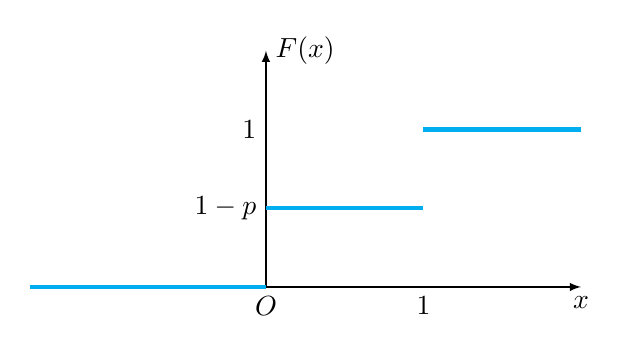
\begin{tikzpicture}[scale = 2]
            %画出x轴,并标注(1,0)
            \draw[-latex] (-1.5,0) -- (2,0) node[below]{$x$};
            \node[left] at (0,1) {$1$} ;
            %画出F(x)轴,并标注(0,0) (0,1) (0,1-p)
            \draw[-latex] (0, 0) -- (0, 1.5) node[right]{$F(x)$};
            \node[below] at (1,0) {$1$};
            \node[left] at (0,0.5) {$1-p$};
            \node[below] at (0,0) {$O$};

            %画出分段的分布函数F(x)
            \draw[cyan, line width = 1.5pt] (-1.5, 0) -- (0, 0);
            \draw[cyan, line width = 1.5pt] (0, 0.5) -- (1, 0.5);
            \draw[cyan, line width = 1.5pt] (1, 1) -- (2, 1);
            %标注虚线连续
            %\draw[dashed, cyan] (0,0) -- (0,0.5);
            %\draw[dashed, cyan] (1,0.5) -- (1,1);
            %标注两个实心连续点
            %\fill[cyan ] (0, 0.5) circle (0.5pt);
            %\fill[cyan ] (1,   1) circle (0.5pt);
            %标注两个空心间断点
            %\draw[cyan ] (0,   0) circle (0.5pt);
            %\fill[white] (0,   0) circle (0.5pt);
            %\draw[cyan ] (1, 0.5) circle (0.5pt);
            %\fill[white] (1, 0.5) circle (0.5pt);
        \end{tikzpicture}
    \end{center}
    (2) 分布函数为
    $$
        F(x) = \begin{dcases}
            0,            & x < 3,             \\
            \frac{1}{10}, & 3 \leqslant x < 4, \\
            \frac{4}{10}, & 4 \leqslant x < 5, \\
            1,            & x \geqslant 5 .
        \end{dcases}
    $$
\end{solution}

\begin{question}{题目20}
    设随机变量 $X$ 的分布函数为
    $$
        F_X(x) = \begin{cases}
            0,      & x<1,                        \\
            \ln{x}, & 1 \leqslant x < \mathrm{e}, \\
            1,      & x \geqslant \mathrm{e}.
        \end{cases}
    $$
    \begin{itemize}
        \item[(1)] 求 $P\{X<2\}$ , $P\{0 < X \leqslant 3\}$ , $P\left\{2 < X < \dfrac{5}{2}\right\}$.
        \item[(2)] 求概率密度 $f_X(x)$.
    \end{itemize}
\end{question}
\begin{solution}
    (1) 根据分布函数的定义
    $$
        P\{X<2\} = F(2) = \ln2.
    $$
    $$
        P\{0 < X \leqslant 3\}
        = P\{X \leqslant 3\} - P\{X \leqslant 0\}
        = F(3) - F(0)
        = 1.
    $$
    $$
        P\left\{2 < X < \frac{5}{2}\right\}
        = P\left\{X<\frac{5}{2}\right\} - P\{X<2\}
        = F\left(\frac{5}{2}\right) - F(2)
        = \ln\frac{5}{4}.
    $$
    (2) 概率密度为
    $$
        f_X(x) = F'_X(x) = \begin{dcases}
            \frac{1}{x}, & 1 \leqslant x < \mathrm{e}, \\
            0,           & \text{其他}.
        \end{dcases}
    $$
\end{solution}


\begin{question}{题目24}
    设顾客在某银行的窗口的等待服务的时间 $X$(min) 服从指数分布,其概率密度为
    $$
        f_X(x) = \begin{dcases}
            \frac{1}{5}\mathrm{e}^{-\frac{x}{5}}, & x>0,         \\
            0,                                    & \text{其他}.
        \end{dcases}
    $$
    某顾客在窗口等待服务,若超过10min他就离开. 他一个月要到银行 $5$ 次. 以 $Y$ 表示一个月内他未等到服务而离开窗口的次数. 写出 $Y$ 的分布律,并求$P\{Y \geqslant 1\}$.
\end{question}
\begin{solution}
    随机变量 $X$ 的分布函数为
    $$
        F_X(x)
        = \int_{-\infty}^{x} f(x) \,\mathrm{d}x
        = \int_{0}^{x} \frac{1}{5}\mathrm{e}^{-\frac{x}{5}} \mathrm{d}x
        = \begin{cases}
            1-\mathrm{e}^{-\frac{x}{5}}, & x>0,         \\
            0,                           & \text{其他}.
        \end{cases}
    $$
    顾客在银行等待时间大于 $10$min 的概率为
    $$
        P\{X>10\} = 1 - P\{X \leqslant 10\}
        = 1 - \left(1-\mathrm{e}^{-2}\right)
        = \mathrm{e}^{-2}.
    $$
    设一个月内顾客有 $k$次因为等待超时而离开窗口,那么 $Y$ 的分布律为
    $$
        P\{Y=k\} = C_5^k\left(\mathrm{e}^{-2}\right)^{k}\left(1-\mathrm{e}^{-2}\right)^{5-k} (k=0,1,2,3,4,5).
    $$
    进一步得到
    $$
        P\{Y \geqslant 1\}
        = 1 - P\{Y=0\}
        = 1 - \left(1-\mathrm{e}^{-2}\right)^5
        \approx 0.5167.
    $$
\end{solution}


\begin{question}{题目27}
    某地区 18 岁的女青年的血压(收缩压以mmHg计)服从 $N(110,12^2)$分布. 在该地区任选一 18 岁的女青年,测量她的血压 $X$. 求
    \begin{itemize}
        \item[(1)] $P\{X \leqslant 105\}$,$P\{100 < X \leqslant 120\}$.
        \item[(2)] 确定最小的 $x$,使 $P\{X>x\} \leqslant 0.05$.
    \end{itemize}
\end{question}
\begin{solution}
    (1) 把正态分布线性变换成标准正态分布,得到
    $$
        \begin{aligned}
            P\{X \leqslant 105\}
             & = P\left\{\frac{X-110}{12} \leqslant \frac{105-110}{12}\right\} \\
             & = \Phi\left(-\frac{5}{12}\right)                                \\
             & = 1 - \Phi\left(\frac{5}{12}\right)                             \\
             & \approx 0.3385.
        \end{aligned}
    $$
    $$
        \begin{aligned}
            P\left\{100 < X \leqslant 120\right\}
             & = P\left\{\frac{100-110}{12} < \frac{X-110}{12} \leqslant \frac{120-110}{12}\right\} \\
             & = \Phi\left(\frac{5}{6}\right) - \Phi\left(-\frac{5}{6}\right)                       \\
             & = 2\Phi\left(\frac{5}{6}\right) - 1                                                  \\
             & \approx 0.5953.
        \end{aligned}
    $$
    (2) 题意等价为 $1 - P\{X \leqslant x\} \leqslant 0.05$ ,再把正态分布线性变换成标准正态分布,得到
    $$
        \begin{aligned}
            P\{X \leqslant x\}                                          & \geqslant 0.95 \\
            P\left\{\frac{X-110}{12} \leqslant \frac{x-110}{12}\right\} & \geqslant 0.95 \\
            \Phi\left(\frac{x-110}{12}\right)                           & \geqslant 0.95 \\
        \end{aligned}
    $$
    查表得到 $\left(\dfrac{x-110}{12}\right)_{\min} = 1.65$,也即 $x_{\min} = 129.8$.
\end{solution}

\begin{question}{题目33}
    设随机变量 $X$ 的分布律为
    $$
        \renewcommand\arraystretch{2}
        \setlength{\arraycolsep}{6mm}
        \begin{array}{c|ccccc}
            X   & -2           & -1           & 0            & 1             & 3              \\
            \hline
            p_k & \dfrac{1}{5} & \dfrac{1}{6} & \dfrac{1}{5} & \dfrac{1}{15} & \dfrac{11}{30} \\
        \end{array}
    $$
    求 $Y=X^2$ 的分布律.
\end{question}
\begin{solution}
    根据
    $$
        P\{Y=0\} = P\{X=0\} = \frac{6}{30}.
    $$
    $$
        P\{Y=1\} = P\{X=-1\} + P\{X=1\} = \frac{7}{30}.
    $$
    $$
        P\{Y=4\} = P\{X=-2\} = \frac{6}{30}.
    $$
    $$
        P\{Y=9\} = P\{X=3\} = \frac{11}{30}.
    $$
    得到 $Y$ 的分布律
    $$
        \renewcommand\arraystretch{2}
        \setlength{\arraycolsep}{6mm}
        \begin{array}{c|cccc}
            X   & 0             & 1             & 4             & 9              \\
            \hline
            p_k & \dfrac{6}{30} & \dfrac{7}{30} & \dfrac{6}{30} & \dfrac{11}{30}
        \end{array}
    $$
\end{solution}


\begin{question}{题目34}
    设随机变量 $X$ 在区间 $(0,1)$ 服从均匀分布.
    \begin{itemize}
        \item [(1)] 求 $Y = \mathrm{e}^X$ 的概率密度.
        \item [(2)] 求 $Y = -2\ln{X}$ 的概率密度.
    \end{itemize}
\end{question}
\begin{solution}
    随机变量 $X$ 在区间 $(0,1)$ 服从均匀分布,概率密度为
    $$
        f(x) = \begin{cases}
            1, & 0<x<1,       \\
            0, & \text{其他}.
        \end{cases}
    $$
    (1) 根据 $Y = \mathrm{e}^X$,得到 $Y$ 的分布函数
    $$
        F_Y(y)
        = P\{Y \leqslant y\}
        = P\left\{\mathrm{e}^X \leqslant y\right\}
        = P\left\{X \leqslant \ln{y}\right\}
        = F_X(\ln{y}).
    $$
    将 $F_Y(y)$ 对 $y$ 求导,得到 $Y = \mathrm{e}^X$ 的概率密度
    $$
        f_Y(y) = F_X'(\ln{y}) = f_X(\ln{y}) \cdot \ln'{y}
        = \begin{dcases}
            \frac{1}{y}, & 0 < \ln{y} < 1, \\
            0,           & \text{其他}.
        \end{dcases}
        = \begin{dcases}
            \frac{1}{y}, & 1 < y < \mathrm{e}, \\
            0,           & \text{其他}.
        \end{dcases}
    $$
    (2) 根据 $Y = -2\ln{X}$,得到 $Y$ 的分布函数
    $$
        F_Y(y)
        = P\{Y \leqslant y\}
        = P\left\{X \geqslant \mathrm{e}^{-\frac{y}{2}}\right\}
        = 1 - P\left\{X < \mathrm{e}^{-\frac{y}{2}}\right\}
        = 1 - F_X\left(\mathrm{e}^{-\frac{y}{2}}\right).
    $$
    将 $F_Y(y)$ 对 $y$ 求导,得到 $Y = -2\ln{X}$ 的概率密度
    $$
        f_Y(y)
        = \left[1 - F_X\left(\mathrm{e}^{-\frac{y}{2}}\right)\right]'
        = -f_X\left(\mathrm{e}^{-\frac{y}{2}}\right) \left(\mathrm{e}^{-\frac{y}{2}}\right)'
        = \begin{dcases}
            \frac{1}{2}\mathrm{e}^{-\frac{y}{2}}, & 0<\mathrm{e}^{-\frac{y}{2}}<1, \\
            0,                                    & \text{其他}.
        \end{dcases}
        = \begin{dcases}
            \frac{1}{2}\mathrm{e}^{-\frac{y}{2}}, & y>0,         \\
            0,                                    & \text{其他}.
        \end{dcases}
    $$
\end{solution}


\begin{question}{题目35}
    设 $X \sim N(0,1)$.
    \begin{itemize}
        \item [(1)] 求 $Y=\mathrm{e}^X$ 的概率密度.
        \item [(2)] 求 $Y=2X^2 + 1$ 的概率密度.
        \item [(3)] 求 $Y=|X|$ 的概率密度.
    \end{itemize}
\end{question}
\begin{solution}
    随机变量 $X \sim N(0,1)$ ,其概率密度为
    $$
        f(x) = \frac{1}{\sqrt{2\pi}}\mathrm{e}^{-\frac{x^2}{2}}.
    $$
    (1) 根据 $Y = \mathrm{e}^X$ 得到 $Y$ 的分布函数
    $$
        F_Y(y)
        = P\{Y \leqslant y\}
        = P\{\mathrm{e}^X \leqslant y\}
        = P\{X \leqslant \ln y\}
        = F_X(\ln{y}).
    $$
    将 $F_Y(y)$ 对 $y$ 求导,得到 $Y=\mathrm{e}^X$ 的概率密度
    $$
        \begin{aligned}
            f_Y(y)
            = F_X'(\ln{y}) = f_X(\ln{y})\cdot\frac{1}{y}
            = \begin{dcases}
                  \frac{1}{\sqrt{2\pi}y}\mathrm{e}^{-\frac{\ln^2y}{2}}, & y > 0,         \\
                  0 ,                                                   & y \leqslant 0.
              \end{dcases}
        \end{aligned}
    $$
    (2) 根据 $Y=2X^2+1$ 得到 $Y$ 的分布函数
    $$
        \begin{aligned}
            F_Y(y)
             & = P\{Y \leqslant y\} = P\{2X^2+1 \leqslant y\}                                     \\
             & = P\left\{-\sqrt{\frac{y-1}{2}} \leqslant X \leqslant \sqrt{\frac{y-1}{2}}\right\} \\
             & = F_X\left(\sqrt{\frac{y-1}{2}}\right) - F_X\left(-\sqrt{\frac{y-1}{2}}\right).    \\
        \end{aligned}
    $$
    将 $F_Y(y)$ 对 $y$ 求导,得到 $Y = 2X^2+1$ 的概率密度
    $$
        \begin{aligned}
            f_Y(y)
             & = F_X'\left(\sqrt{\frac{y-1}{2}}\right)
            - F_X'\left(\sqrt{\frac{y-1}{2}}\right)                                              \\
             & = f_X\left(\sqrt{\frac{y-1}{2}}\right)\left(\sqrt{\frac{y-1}{2}}\right)'
            - f_X\left(-\sqrt{\frac{y-1}{2}}\right)\left(-\sqrt{\frac{y-1}{2}}\right)'           \\
             & = \begin{dcases}
                     \frac{1}{2\sqrt{\pi(y-1)}}\mathrm{e}^{-\frac{y-1}{4}}, & y \geqslant 1, \\
                     0,                                                     & \text{其他}.
                 \end{dcases}
        \end{aligned}
    $$
    (3) 根据 $Y=|X|$ 得到 $Y$ 的分布函数
    $$
        F_Y(y) = P\{Y \leqslant y\}
        = P\{|X| \leqslant y\}
        = P\{-y \leqslant X \leqslant y\}
        = F_X(y) - F_X(-y).
    $$
    将 $F_Y(y)$ 对 $y$ 求导,得到 $Y = |X|$ 的概率密度
    $$
        f_Y(y) = F_X'(y) - F_X'(-y)
        = f_X(y) - [-f_X(-y)]
        = \begin{dcases}
            \sqrt{\frac{2}{\pi}}\mathrm{e}^{-\frac{y^2}{2}}, & y \geqslant 0, \\
            0,                                               & \text{其他}.
        \end{dcases}
    $$
\end{solution}